\chapter{Experiments}\label{chap:experiments}

Cloud computing is a change and if used in the right way, can be a great accelerator of collaborated architecture. Cloud is an Internet phenomenon and trying to use cloud the traditional enterprise way will not achieve real returns from the cloud. In short Enterprises need to embrace new architecture. 

One approach is using an incremental approach. This is less risky than big-bang and also gives transition time to employees. This approach uses a hybrid cloud where existing on-prem resources are connected to new resources on cloud. New external cloud services can be incorporated in the in-house solutions, leading way to gradually get rid of on-prem resources by their end of life. 

Consider a basic on-prem architecture.

\begin{figure}[!htb]
    \center{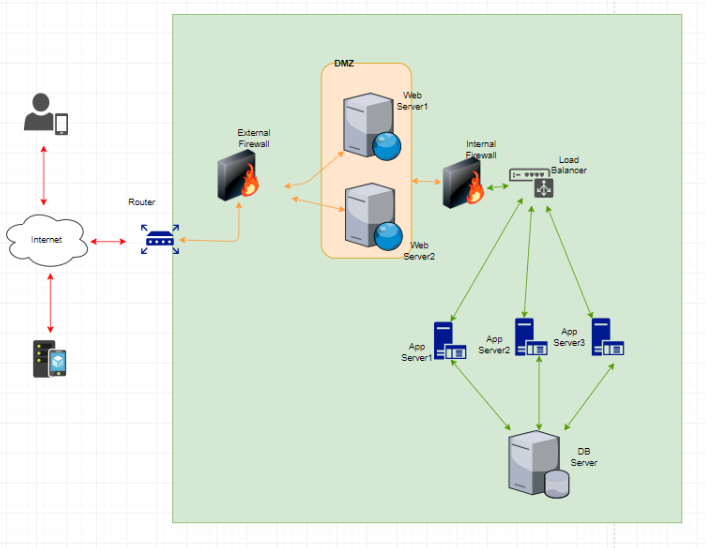
\includegraphics[width=0.5\textwidth]
    {figures/experiments/General_Cloud_Architecture.png}}
    \caption{\label{fig:GCA} General Cloud Architecture}
\end{figure}

\section{Azure Data Factory and SQL Database}
As part of our experiment we want to move compute to Azure Cloud by using Azure Data Factory. Azure Data Factory is a fully managed service provided by Microsoft that composes data storage, processing and movement services into streamlined, scalable, and reliable data production pipelines. To utilize compute in Azure Cloud we have created table sales\_records in Azure SQL Database Cloud and an SSIS service in AzureDataFactory. Once SSIS service is deployed to Cloud it is scheduled to be run daily which computes sales data for every quarter and sales for every product based on region. We are utilizing database in cloud due to the limitations of creating VPN or direct-connect as these seem to be costly options for an individual, but any corporation or industry will have VPN or direct-connect set to reduce latency. Corporation can use VPN or direct-connect to connect to on-premises database.

\begin{figure}[!htb]
    \center{\includegraphics[width=0.5\textwidth]
    {figures/experiments/SSIS_ADF.png}}
    \caption{\label{fig:SSIS_ADF} SSIS Azure Data Factory}
\end{figure}
%\begin{center}
%\includegraphics[scale=0.5]{SSIS_ADF.png}
%\end{center}

\begin{enumerate}
 \item Create SQL Database. 
 \begin{enumerate}
 	\item Login to Azure portal and click create SQL Database
	\item Create Cloud Computing database with a blank database
	\item Once DB is created, get the connection string for this database.
 \end{enumerate}  
 \item Create Azure Data Factory. 
 \begin{enumerate}
 	\item Login to Azure portal and click Data + Analytics and click Data Factory
	\item Create unique name for SSIS Data Factory
	\item Click Author and Monitor.
	\item Click Configure SSIS Integration Runtime tile.
	\item On the SQL Settings page enter the configuration of the above SQL Database.
	\item Select Catalog Database Server Endpoint to host SSISDB.
 \end{enumerate}  
\end{enumerate}
 
\section{S3 --> Lambda --> DynamoDB}
As part of this experiment we upload a csv file to S3. AWS Lambda has a trigger whenever a new item is added to S3. Lambda function kicks in, it does its processing and uploads the data in csv file in S3 to DynamoDB. DynamoDB can process this data for end user or any analytic requirement. AWS Lambda is a serverless architecture which utilizes resources required for processing the file in S3 to DynamoDB. Once the processing is complete the client is not charged unless the Lambda function is triggered again. To achieve this we followed the following steps: \cite{ReadCSVFile}

\begin{figure}[!htb]
    \center{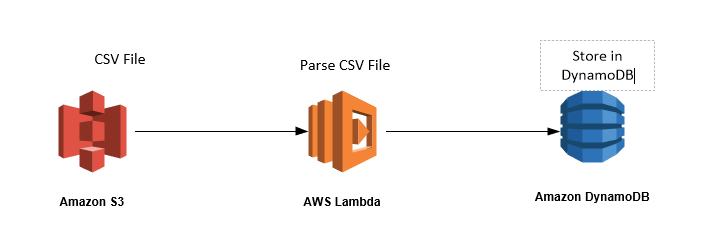
\includegraphics[width=0.5\textwidth]
    {figures/experiments/AWS_S3_Lambda_DynamoDB.png}}
    \caption{\label{fig:S3_DynamoDB} AWS Lambda S3 to DynamoDB}
\end{figure}
%\begin{center}
%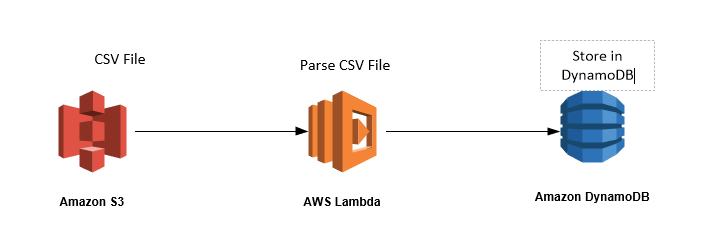
\includegraphics[scale=0.75]{figures/experiments/AWS_S3_Lambda_DynamoDB.png}
%\end{center}

\begin{enumerate}
 \item Create Policy in IAM. 
 \begin{enumerate}
 	\item Select S3, then select all actions and all resources
	\item Add additional permissions for DynamoDB, select all actions and all resources
	\item Add additional permissions for Cloudwatch, select all actions and all resources.
 \end{enumerate}  
 \item Create Role
 \begin{enumerate}
 	\item Attach the above policy to this role
\end{enumerate}
 \item Create Lambda Function
 \begin{enumerate} 
 	\item Create function, author from scratch
 	\item Give function name
 	\item Select runtime as Python 3.0
 	\item Choose existing role
 	\item Select role created above
 	\item Add trigger for S3, select bucket, event type (object created), prefix and filter if any.
 \end{enumerate}
\end{enumerate}

\section{AWS/Google Cloud --> Azure SQL Database}
As part of this experiment we connected AWS EC2/Google Compute instance to Azure SQL Database.

\begin{center}
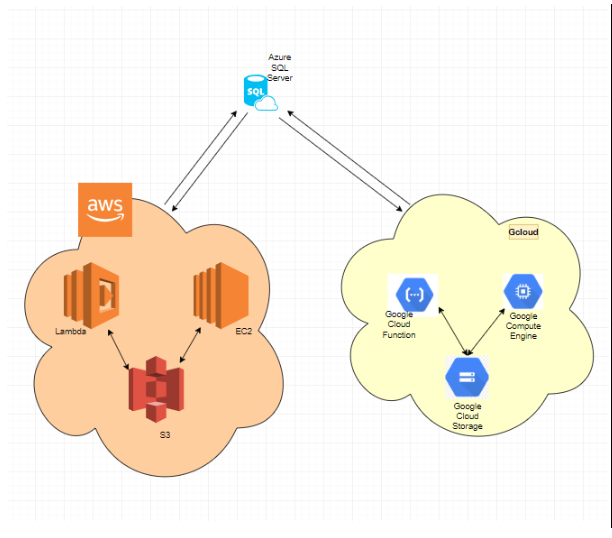
\includegraphics[scale=0.75]{figures/experiments/AWS_Google_to_AzureDB.png}
\end{center}

\subsection{Operations}
 \begin{enumerate} 
 	\item Connect to Azure SQL Server 
 	\item Load a file
 	\item Read a table from Azure SQL server 
 \end{enumerate}

